%# -*- coding:utf-8 -*-
%告诉编辑器以utf-8的模式打开该文档
\documentclass{paper}

\usepackage{geometry}
\usepackage{float} %ͼƬ����
%\usepackage[section]{placeins} %���⸡������ \section
\usepackage{placeins}
\usepackage{array}
\usepackage{setspace} %���ü��
\usepackage{fontspec} %���������
\setmainfont{Times New Roman} %������������
\setCJKmainfont{SimSun} %������������
\geometry{a4paper,top=2.54cm,bottom=2.54cm,left=3.17cm,right=3.17cm,head=1.57cm,foot=1.5cm}

%�����ʽ
\newcommand{\PreserveBackslash}[1]{\let\temp=\\#1\let\\=\temp}
\newcolumntype{C}[1]{>{\PreserveBackslash\centering}p{#1}}
\newcolumntype{R}[1]{>{\PreserveBackslash\raggedleft}p{#1}}
\newcolumntype{L}[1]{>{\PreserveBackslash\raggedright}p{#1}}
 %导入导言区内容

\begin{document}
\titleformat{\chapter}{\vspace*{-5.5em}\centering\heiti\zihao{-3}\bfseries}{第\,\chaptername 章}{1em}{\vspace{0em}}

\graphicspath{{figures/}}

%封面
%# -*- coding:utf-8 -*-
%论文封面
\title{银行客户关系管理信息系统的设计与实现}
\entitle{Design and Implementation of the Customer Relationship Management Information System for Banks}
\author{黄亚磊}
\idn{30920111242116}
\degree{硕}
\teacher{周\s 理\s 成\s 教\s 授}
\subject{纳\s 米\s 材\s 料\s 科\s 学}
\subdate{2017\s 年\s 4\s 月}
\defdate{2017\s 年\s 5\s 月}
\oftdate{2017\s 年\s 6\s 月}

\pubdate{2017年4月}
\maketitle

%英文封面,不需要的话可去掉以下代码
\engdegree{Master of Science}
\enauthor{Yalei Huang }
\enteacher{Prof. Licheng Zhou}
\enschool{Department of Chemistry}
\enpubdate{April,2017}

\makeencover



%声明
%# -*- coding:utf-8 -*-
\pagestyle{empty}
%\begin{document}
%\fontsize{14}{21}\selectfont
\section*{\centering\heiti \zihao{-2}厦门大学学位论文原创性声明}
\vspace{21pt}
 \par \zihao{4}
 本人呈交的学位论文是本人在导师指导下,独立完成的研究成果。本人在论文写作中参考其他个人或集体已经发表的研究成果,均在文中以适当方式明确标明,并符合法律规范和《厦门大学研究生学术活动规范(试行)》。
 \par
 另外,该学位论文为(\hspace{12em})课题(组)的研究成果,获得(~~~~~~~~~~~~~~~~~~~~~~~~~~~)课题(组)经费或实验室的资助,在(~~~~~~~~~~~~~~~~~~~~~~~~~~~~~~~~~~)实验室完成。(请在以上括号内填写课题或课题组负责人或实验室名称,未有此项声明内容的,可以不作特别声明。)
 \par
 本人声明该学位论文不存在剽窃、抄袭等学术不端行为,并愿意承担因学术不端行为所带来的一切后果和法律责任。
 \vspace{3ex}
 \par \hfill
 声明人(签名):~~~~~~~~~~~~
\par \hfill
 指导教师(签名):~~~~~~~~~~~~
 \par \hfill
 年~~~~~~~~月~~~~~~~~~日
 \clearpage\cleardoublepage

\section*{\centering\heiti \zihao{-2}厦门大学学位论文著作权使用声明}
\vspace*{21pt}
 \par
 本人同意厦门大学根据《中华人民共和国学位条例暂行实施办法》等规定保留和使用此学位论文,并向主管部门或其指定机构送交学位论文(包括纸质版和电子版),允许学位论文进入厦门大学图书馆及其数据库被查阅、借阅。本人同意厦门大学将学位论文加入全国博士、硕士学位论文共建单位数据库进行检索,将学位论文的标题和摘要汇编出版,采用影印、缩印或者其它方式合理复制学位论文。
 \par
 本学位论文属于:
 \par
 (~~~~~)1.经厦门大学保密委员会审查核定的保密学位论文,于~~~~~~年~~~~月~~~~日解密,解密后适用上述授权。
 \par
 (~~√~~)2.不保密,适用上述授权。
 \par
 (请在以上相应括号内打“√”或填上相应内容。保密学位论文应是已经厦门大学保密委员会审定过的学位论文,未经厦门大学保密委员会审定的学位论文均为公开学位论文。此声明栏不填写的,默认为公开学位论文,均适用上述授权。)
 \vspace{3ex}
 \par \hfill
 声明人(签名):~~~~~~~~~~~~
 \par \hfill
 年~~~~~~~~月~~~~~~~~~日



\zihao{-4}
%摘要
 %# -*- coding:utf-8 -*-
\pagenumbering{Roman} %定义页码格式为罗马字母
\begin{cabstract}
%[客户关系管理;银行;J2EE平台;数据仓库]
客户关系管理(Customer Relationship Management,简称CRM)作为一种新的管理模式、业务营销理念和信息技术前沿产品,是信息技术与业务管理相结合的产物。银行客户关系管理是指商业银行树立以客户为中心的经营理念,在准确市场定位的基础上合理配置资源,发现并最大限度满足优质客户的需要,持续进行流程优化和金融创新,充分发挥客户经理的积极性,在提高客户价值的过程中实现银行自身价值的提升。

本文首先介绍了银行建立CRM系统的必要性,CRM系统对银行带来的帮助。然后对银行CRM系统进行了需求分析,设计出了银行CRM系统的架构,由三层结构组成,一是数据源层,二是数据仓库分析层,三是界面表示层。其中数据仓库分析层是整个CRM系统的核心。接着本文介绍了开发银行CRM系统的相关技术,采用的是J2EE平台,使用Struts 2,Spring,Hibernate的框架。最后把实现的CRM系统的部分界面截图,以及相关的一些关键代码呈现了出来。
\keywords{客户关系管理;银行;J2EE平台;数据仓库}

\end{cabstract}

\begin{eabstract}
Customer relationship management(CRM),an updated product of a new management model,a business marketing concept and information technology, is regarded as a combination of information technology and business management,which has attracted the attention of management of banking community ever since.Bank CRM means to establish a customer-centric management concept for commercial banks,allocate the resources on the basis of accurate market orientation,enhance the customer managers’ initiatives and realize the upgrading of bank self-value.

   Firstly, this paper introduces the need for banks to establish a CRM system, CRM system for banks to help. Then, Bank CRM system requirements analysis, design the architecture of the bank CRM system, consisting of three-layer structure, one data source layer, is the analysis of the data warehouse layer, interface presentation layer. The data warehouse analysis layer is the core of the CRM system as a whole. Then the article describes the bank's CRM system technology, using the J2EE platform using Struts 2, Spring, Hibernate framework. Finally, the CRM system to achieve some interface screen shots, and some of the key code presents.
\ekeywords{CRM; Bank; J2EE Platform; Data Warehouse}
\end{eabstract}

%生成中文目录
\tableofcontents

%生成英文目录
\tableofengcontents

%章节
%# -*- coding:utf-8 -*-
\pagenumbering{arabic}
\chapter{绪论}
\echapter{Introduction}
\section {研究背景和意义}
\esection{Research Background and Significances}
国内外有很多组织都已经开展了CRM的研究和开发工作,从管理到技术都有。在市场上,也开发了不少的CRM产品。虽然CRM产品具有各种不同规模,不同功能等特性,但是从其主要的功能特性上区分,CRM 产品可以分为以下几种
\subsection{国内外研究现状}
\esubsection{Research Status at Home and Abroad}
经过十几年金融电子化的改造,银行业经历了脱机业务处理,联机业务处理,数据集中处理。随着银行业网络化服务和管理信息化,业务虚拟化时代的来临。数据大集中告别手工的电子化后,为下一步进行信息化,利用数据仓库和管理系统把数据转化为有用的信息以支持管理决策,并最终实现知识化提供了信息基础\footnote{韩愈(768-824),字退之,河南河阳(
  今河南孟县)人,自称郡望昌黎,世称韩昌黎。幼孤贫刻苦好学,德宗贞元八年进士。}。数据大集中后实时业务处理系统较为先进和方便,但尚缺乏强大的业务支持管理系统,而这正是中国银行金融企业全面管理集中,全面成本控制,全面客户服务,全面风险防范和全面面向未来所必需的,如公式\ref{equ1}。
  \begin{equation}\label{equ1}
    \hat{a}+\hat{a}=\sqrt{{ab}^2}+\sqrt[n]{abc}
  \end{equation}

当今世界经济正朝着全球市场一体化,企业生存数字化,商业竞争国际化的方向发展,在这样的大背景下,以互联网,知识经济,高薪技术为代表,以满足客户的需求为核心的新经济迅速发展开来。在这新经济时代,企业的产品服务不再是竞争的核心,客户成为决定企业胜败的关键,这使得对客户关系管理的研究兴起,如表\ref{dataT}。
\renewcommand\arraystretch{1.5}
\begin{table}[!htb]
\centering
\caption{基本资料表}
\label{dataT}
\begin{tabular}{|l|l|l|l|l|}
\hline
\textbf{字段名称} & \textbf{字段类型} & \textbf{长度} & \textbf{字段描述} & \textbf{备注} \\ \hline
账户号           & Number        & 30          &               & 主键          \\ \hline
密码            & Number        & 30          & 加密            &             \\ \hline
姓名            & Varchar       & 50          &               &             \\ \hline
电子邮箱          & Varchar       & 50          & VIP客户必填       &             \\ \hline
\end{tabular}
\end{table}


银行服务的营销理念转成以客户为中心也有一个发展过程,在以前的时候,我国的商业银行,特别是国有商业银行,可以称为是“皇帝的女儿” ,各系统设置都是以账户为中心,为社会提供的银行服务都是有限的,品种单一的,对老百姓和机构都是一视同仁,无所谓“优质”服务与否,没有客户是否满意的概念,用来衡量银行经营目标和员工工作目标完成情况的重要指标\footnote{曾任监察御史,因上疏请免关中赋役,贬为阳山县令。后随宰相裴度平定淮西迁刑部侍郎,又因上表谏迎佛骨,贬潮州刺史。做过吏部侍郎,死谥文公,故世称韩吏部、韩文公。是唐代古文运动领袖,与柳宗元合称韩柳。诗力求险怪新奇,雄浑重气势。}。而如今日益激烈和全球化的竞争使银行逐渐认识到:银行的资产状况越来越取决于客户的状况,而要维系老客户,争取新客户以保持银行的竞争力,就必须融入CRM(Customer Relationship Management, 客户关系管理)的管理理念并建立相应的CRM系统,如公式\ref{equ2}。
\begin{align}\label{equ2}
  x&\equiv y+1(mod ~m^{2}) \\
  x&\equiv y+1mod ~m^{2} \nonumber \\
  x&\equiv y+1(m^{2}) \nonumber
\end{align}

最近10年来,全球化的竞争格局迫使商业银行不断扩展业务范围,而在技术水平相差不大的情况下,竞争也就聚焦在高效益的客户上。客户状况决定着银行的资产状况,具有良好发展前途的优质客户是银行优质资产的源泉,因此,客户是银行最重要的资源,银行对客户需求的满足能力是银行能否与客户保持紧密联系,获得发展的关键所在。在这样的情况下,越来越多的银行开始认识并引进

\section{国内外研究现状}
\esection{Research Status at Home and Abroad}
目前,国内外有很多组织都已经开展了CRM的研究和开发工作,从管理到技术都有。在市场上,也开发了不少的CRM产品。虽然CRM产品具有各种不同规模,不同功能等特性,但是从其主要的功能特性上区分,CRM产品\ucite{qzm2008}可以分为以下几种

1.	传统ERP型\ucite{djh2011}

传统ERP型CRM产品主要是许多主要的传统后端ERP厂商,如Oracle, SAP, PeopleSoft 等,进入CRM 市场所开发的CRM产品。该类产品的最大特点是采用了客户智能,融会贯通的交流渠道和基于Internet 技术的应用体系结构。其中客户智能是指该产品拥有强健的信息处理和商业分析能力,能够跨越多个软件模块和业务单位,对客户进行全面和智能的分析。融会贯通的交流渠道是指该产品将多种客户交流渠道集成起来,使各种渠道融会贯通,以保证企业,客户都能得到完整,准确和一致的信息。该类型的产品尤其以Oracle Application 为代表,如图\ref{f1}。
\begin{figure}[htb]
  \centering
  % Requires \usepackage{graphicx}
  
\includegraphics[width=10cm]{1.jpg}\\
  \caption{图片1}\label{f1}
\end{figure}


2.	数据分析型\ucite{tfp}

数据分析型CRM产品认为数据仓库是进行客户分析的基础。数据仓库所建立的客户数据库使企业能收集到更详细的客户信息档案,以便对现有客户提供更好的服务,也可以建立一个预测模型,尽可能准确地预报客户流失的概率和可能性,以便及早采取相应的措施。利用数据挖掘工具和统计模型对数据仓库的数据进行研究,可以分析顾客的购买习惯,广告成功率和其他战略性的信息。这里恶性的产品是以Wal-Mart公司的数据仓库为代表。

\section{研究目的和研究内容}
\esection{Research aims and content}
本文的研究目的在于开发的CRM系统以及相关的数据仓库平台,使银行金融,信贷,决策,推广等部门更方便快捷准确有效的制定目标决策规划,并找出目标重点客户,进行按各个行业,各个产品,主要客户等各个层次的效益分析。业务部门依据各种报表,为客户提供一对一的贴心服务,同时为银行领导和金融部门的快速决策提供了良好的支持,提高了银行整体的竞争力,如图\ref{f2}。
\begin{figure}[htbp]
  \centering
  % Requires \usepackage{graphicx}
  
\includegraphics[width=8cm]{2.jpg}\\
  \caption{图片2}\label{f2}
\end{figure}


本文意在实现一个CRM系统,该系统根据客户关系管理理论应具备的三大子系统,分别为营销管理子系统,销售管理子系统,服务管理子系统。主要实现以下几点:

1. 建设管理信息体系架构。通过技术手段,把现有的各种业务经营和服务渠道系统资源联系在一起,通过对信息的采集,提炼,建议起管理信息平台。

2. 为营销提供资料,使客户忠诚度得到提高。对客户进行评价,发现优质客户,重点发展该种客户,维持好客户的良好关系,提高客户重复交易行为。

3. 发展新客户.发展新的客户关系,了解不同客户的不同需求,提高客户满意度,进而发挥最大的促销能力,增加业务量,提高经济效益。

4. 减少成本。通过技术与业务流程的整合,精简业务流程,防范业务操作风险,节省成本。

5. 减少成本。通过技术与业务流程的整合,精简业务流程,防范业务操作风险,节省成本。

\section{本文组织结构}
\esection{Outline of the Dissertation}
全文共分为五章:

第1章是绪论,主要介绍了系统的研究目的和意义,以及国内外的研究现状。

第2章是相关技术介绍,对本系统实现所涉及到的一些框架和技术进行了简单的介绍。

第3章是系统需求分析,对系统进行概述,并对其需求进行分解,对系统的整个架构进行了分析。

第4章是系统设计,分析了系统的设计原则和目标,介绍了系统技术构架设计,并给出了系统的总体功能架构图,同时对系统项目管理设计也做了一定的介绍。

第5章是系统实现,对系统的界面、业务、工作流等方面做了实现功能的描述。列出了一些关键的相关代码。

第6章总结与展望部分,对本文进行了总结,并对下一步的工作进行了展望。






\chapter{系统相关技术}
\echapter{Introduction of System Related Technologies}
\section{J2EE的开发框架}
\esection{J2EE development framework}
J2EE技术自从被推出以来就得到了广泛认可和应用,随着多年的技术演变和发展,J2EE技术平台已经日趋成熟,成为当今电子商务的最佳解决方案。相对于微软推出的.NET平台,J2EE继承了Java平台无关性的优点,成为金融,保险,电信等大型应用系统的首选平台方案,如图\ref{2bro}所示。
\begin{figure}[htbp]
  \centering
  % Requires \usepackage{graphicx}
  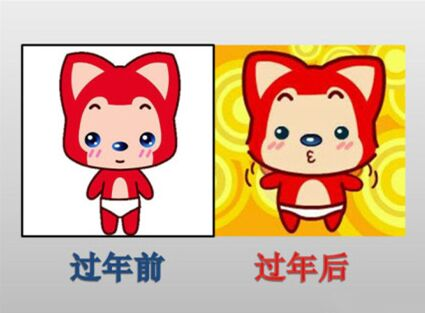
\includegraphics[width=10cm]{3.jpg}\\
  \caption{搞笑图片}\label{2bro}
\end{figure}
\subsection{Struts 2}
\esubsection{Struts 2}
Struts 2最早是Apache Jakarta项目的组成部分,项目创立者希望通过对该项目的研究,改进和提高JSP,Servlet, 标签库以及面向对象的技术水准。 Struts 2采用MVC模式,帮助JAVA开发者利用J2EE开发WEB应用。和其他JAVA架构一样,Struts2也是面向对象的设计,充分发挥了MVC模式 “分离显示逻辑和业务逻辑”的优势。

\renewcommand\arraystretch{1.2}
\begin{table}[htb]
\centering
\caption{My caption}
\label{my-label}
\begin{tabular}{llr}
\hline
\multicolumn{2}{c}{Item} &            \\ \cline{1-2}
Animal     & Description & Price (\$) \\ \hline
Gnat       & per gram    & 13.65      \\
           & each        & 0.01       \\
Gnu        & stuffed     & 92.50      \\
Emu        & stuffed     & 33.33      \\
Armadillo  & frozen      & 8.99       \\ \hline
\end{tabular}
\end{table}

\FloatBarrier
\subsection{Hibernate概述}
\esubsection{Introduction of Hibernate}
Hibernate 是一个开放源代码的对象关系映射框架,对JDBC进行了轻量级的对象封装,使得JAVA程序员可以使用对象编程思维来操作数据库,可以应用在任何使用JDBC的场合,可以在JAVA客户端程序中使用,也可以在Servlet/JSP的Web应用中使用,最厉害的是,它可以在应用EJB的J2EE架构中取代CMP(容器管理持久化),完成数据持久化的重任。


\section{数据库技术}
\esection{Introduction of Database Access Technology}
本文所使用的数据库为开源的MYSQL,MYSQL是一个小型关系数据库管理系统,该数据库的用户已经成千上万了。在本文所实现的CRM系统中需要使用数据库的关键技术就是数据仓库。

数据仓库也是一个数据库,并且大部分都是基于关系型数据库管理系统(RDBMS)设计的,和服务于特定应用软件的交易型数据库不同。数据仓库精简并整合了企业多个数据源的原始数据,其主要用途是为数据访问和企业分析决策之用。数据仓库的整个数据库同交易型数据库是分开的,是各种数据分析工具,信息显示系统的“数据源”,而交易型数据库则是数据仓库的数据源。
\begin{figure}
  \centering%
  \subfigure[第一个小图形]{%
    \label{fig:subfig1}
    
\includegraphics[height=5cm]{4.jpg}}%
  \subfigure[第二个小图形]{%
    \label{fig:subfig2}
    
\includegraphics[height=5cm]{5.jpg}}
  \caption{包含子图形的大图形}
  \label{fig:big1}
\end{figure}

数据仓库虽然同一般交易型数据库采用同样的关系数据库管理系统,但由于建库的目的不同,在设计上是有区别的。在性能上,数据仓库要求快速查询和统计计算,而交易型数据库则要求快速插入或更新,如表\ref{tbl1}所示。
\renewcommand\arraystretch{1.5}
\begin{table}[hbtp]
\centering
\caption{分析型与交易型比较}
\label{tbl1}
\begin{tabular}{|p{3cm}<{\raggedright}|p{5.5cm}<{\raggedright}|}
%\begin{tabular}{|C{3cm}|C{5.5cm}|}
\hline
 & \multicolumn{1}{c|}{\textbf{实体关系特征}} \\ \hline
\textbf{\PreserveBackslash 分析型数据仓库} & 较少连接简单的星型关系链 \\ \hline
\textbf{交易型数据库} & 关系复杂,很多连接 \\ \hline
\end{tabular}
\end{table}


\FloatBarrier
\section{本章小结}
\esection{Summary}
本章主要对本文所实现的银行CRM系统运用的相关关键技术进行了一定的介绍,该系统使用瘦客户端的B/S架构,在J2EE平台上实现。具体的平台使用的是MyEclipse 6.0.所使用的架构是Struts 2+Hibernate+Spring, Struts 2负责MVC模型的建立,Hibernate能让用户用面向对象的思维操作数据库,Spring可以使用JavaBean来完成以前只能由EJB完成的工作。服务器使用的是Apache。


%研究成果
%# -*- coding:utf-8 -*-
\begin{publications}
[1] 作者列表.论文题目.期刊名称,期刊号(编号),起始页码,年份.

[2] 杨怡,贾泽.用于雅典和电容微麦克风的体硅腐蚀相关研究.压电与声光,2006,28(1):117-119.
\end{publications}


%参考文献
%# -*- coding:utf-8 -*-
\begin{xmuref}
 %\bibliographystyle{unsrt}
 %\bibliography{ref/refs}
 \bibliographystyle{XMU} %格式文件
 \bibliography{ref/paper}%bib文件
\end{xmuref}


%致谢
\begin{ack}
阳春三月,在完成硕士论文的这个激动人心的时刻,回眸硕士研究生的学习生活,心中不禁感慨万千。在这里。我首先要感谢我的父母。正是由于他们那无私的爱和无比的耐心和宽容才使得我能够健康而快乐地成长。在此,我向他们表达我最诚挚的敬意和最真诚的爱。

在他的悉心指导下,我的开发设计才工作得以顺利进行,在技术上大有长进,在研究方法上大受裨益。在读期间,导师都给予了谆谆教导和亲切关怀,为我的学习和工作提供了良好的软硬件条件。从毕业论文选题开始、开发设计工作的开展到论文的最后完成,都倾注了导师大量的心血,在本论文的撰写和定稿过程中,导师提出了许多宝贵、中肯的意见。在此,特向教授致以最诚挚的敬意和最衷心的感谢。
\end{ack}


\end{document}
